\documentclass{beamer}
\usepackage{graphicx} % Required for inserting images

\usepackage[utf8]{inputenc}
\usepackage[T1]{fontenc}
\usepackage{lmodern}
\usepackage{amsmath,amssymb}
\usepackage{microtype}
\usepackage{ellipsis}
%\usepackage[ngerman]{babel}
\let\openbox\undefined
\usepackage{mathtools}
\usepackage{enumitem}
\let\openbox\undefined
\usepackage{amsthm}
\usepackage{thmtools}
\usepackage{graphicx}
\usepackage{stmaryrd}
\usepackage{tikz}
\usetikzlibrary{positioning}
\usepackage{algpseudocode}
\usepackage[absolute,overlay]{textpos}
\usepackage{url}
\usepackage[
backend=biber,
style=numeric,
]{biblatex}
\addbibresource{references.bib}
\usepackage[normalem]{ulem}

\declaretheoremstyle[
    headpunct=,
    spacebelow=2em,
    spaceabove=1em,
    postheadspace=\newline,
    ]{aufgabe}
\declaretheorem[style=aufgabe]{aufgabe}
\numberwithin{equation}{aufgabe}
\addtolength\jot{1ex}

\newtheorem{proposition}{Proposition}
\renewcommand\qedsymbol{$\square$}

\newcommand\R{\mathbb R}
\newcommand\Z{\mathbb Z}
\newcommand\N{\mathbb N}
\newcommand\C{\mathbb C}
\newcommand{\Q}{\mathbb Q}
\newcommand{\F}{\mathbb{F}}
\newcommand{\ass}{\underline{Assume:}  }
\newcommand{\zz}{\underline{t.s.:}  }

\usetheme[compress]{Berlin}
\setbeamertemplate{footline}[frame number]{}
\setbeamertemplate{navigation symbols}{}
\setbeamertemplate{footline}{}

\makeatletter
\beamer@theme@subsectionfalse%
\makeatother

\title{Deep Learning}
\author{Lukas Schnelle}
\date{June 2023}

\begin{document}

\maketitle

\section{Problem statement}
\begin{frame}{An Example}
    \visible<2-4>{
    Let $\forall i \in [n]: a_i \in \R^1, b_i \in \R $ some data.\\
    \textbf{Goal:} Find $x \in \R$ s.th. $ax \only<3-4>{\textcolor{red}{\leq}} \only<2>{=} -b$}
    \only<1-3>{
    \begin{center}
        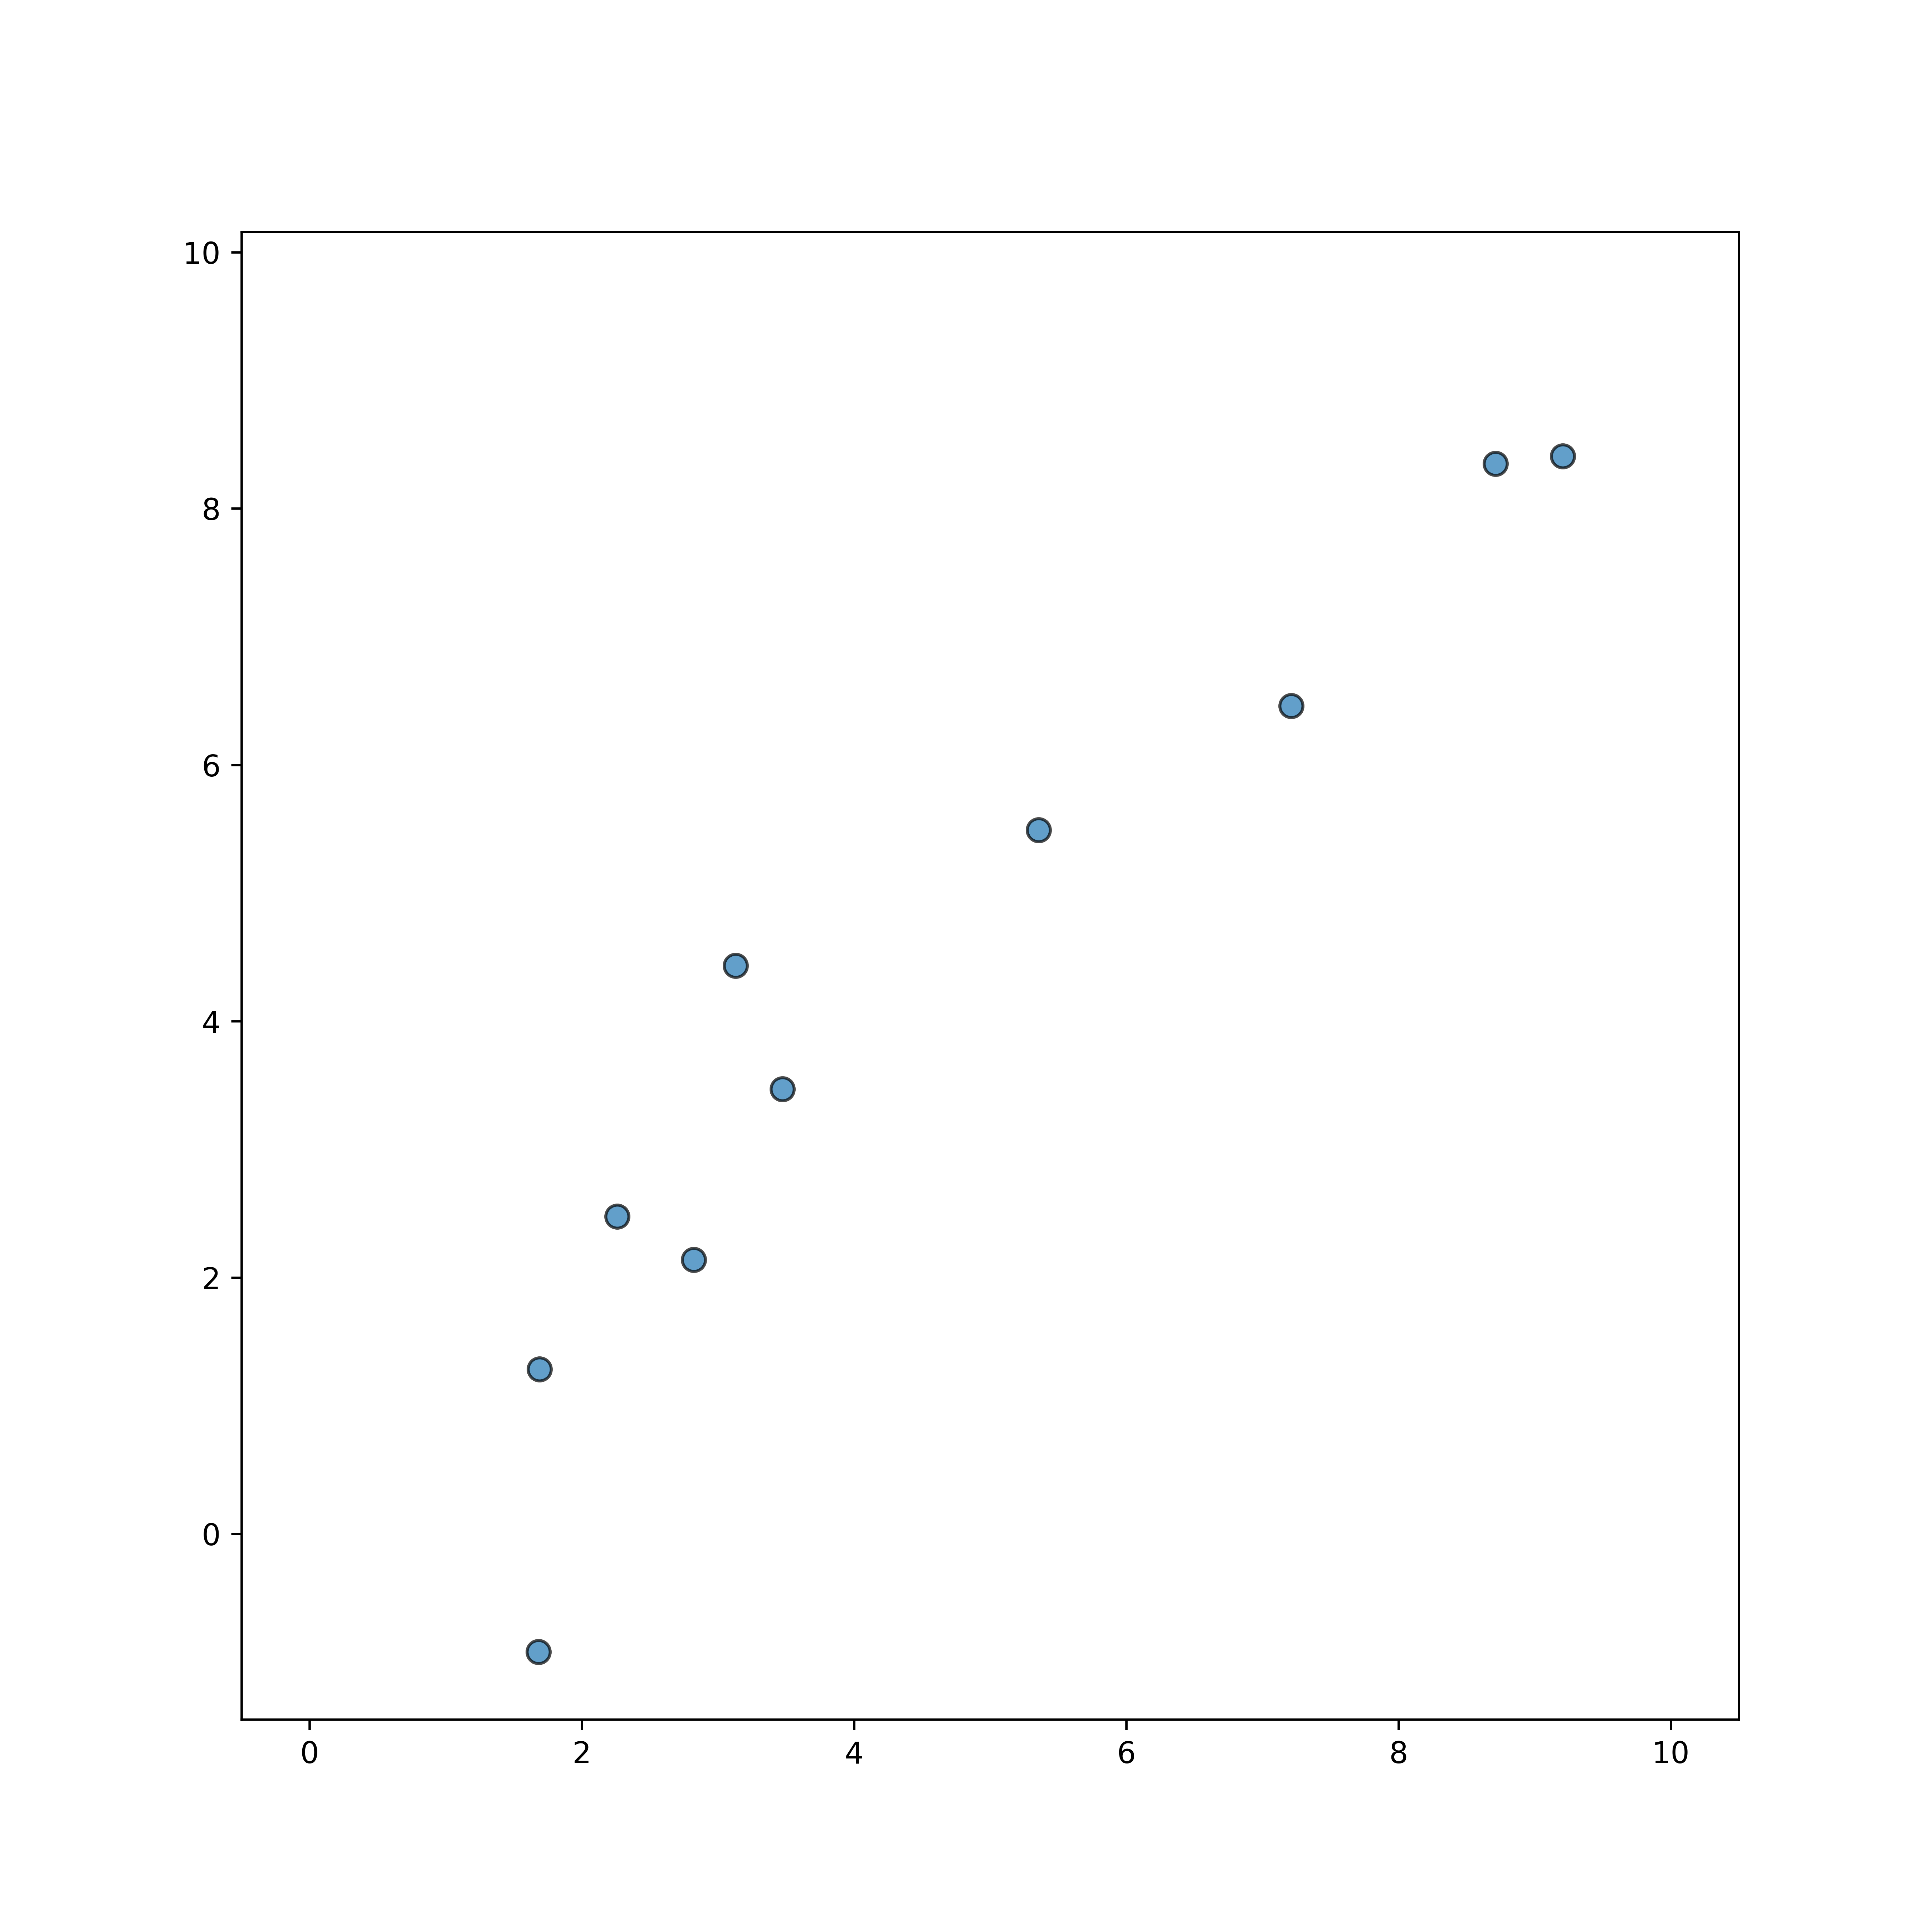
\includegraphics[width=0.6\textwidth]{images/pointplot.png}
    \end{center}
    }
    \only<4>{
    \begin{center}
        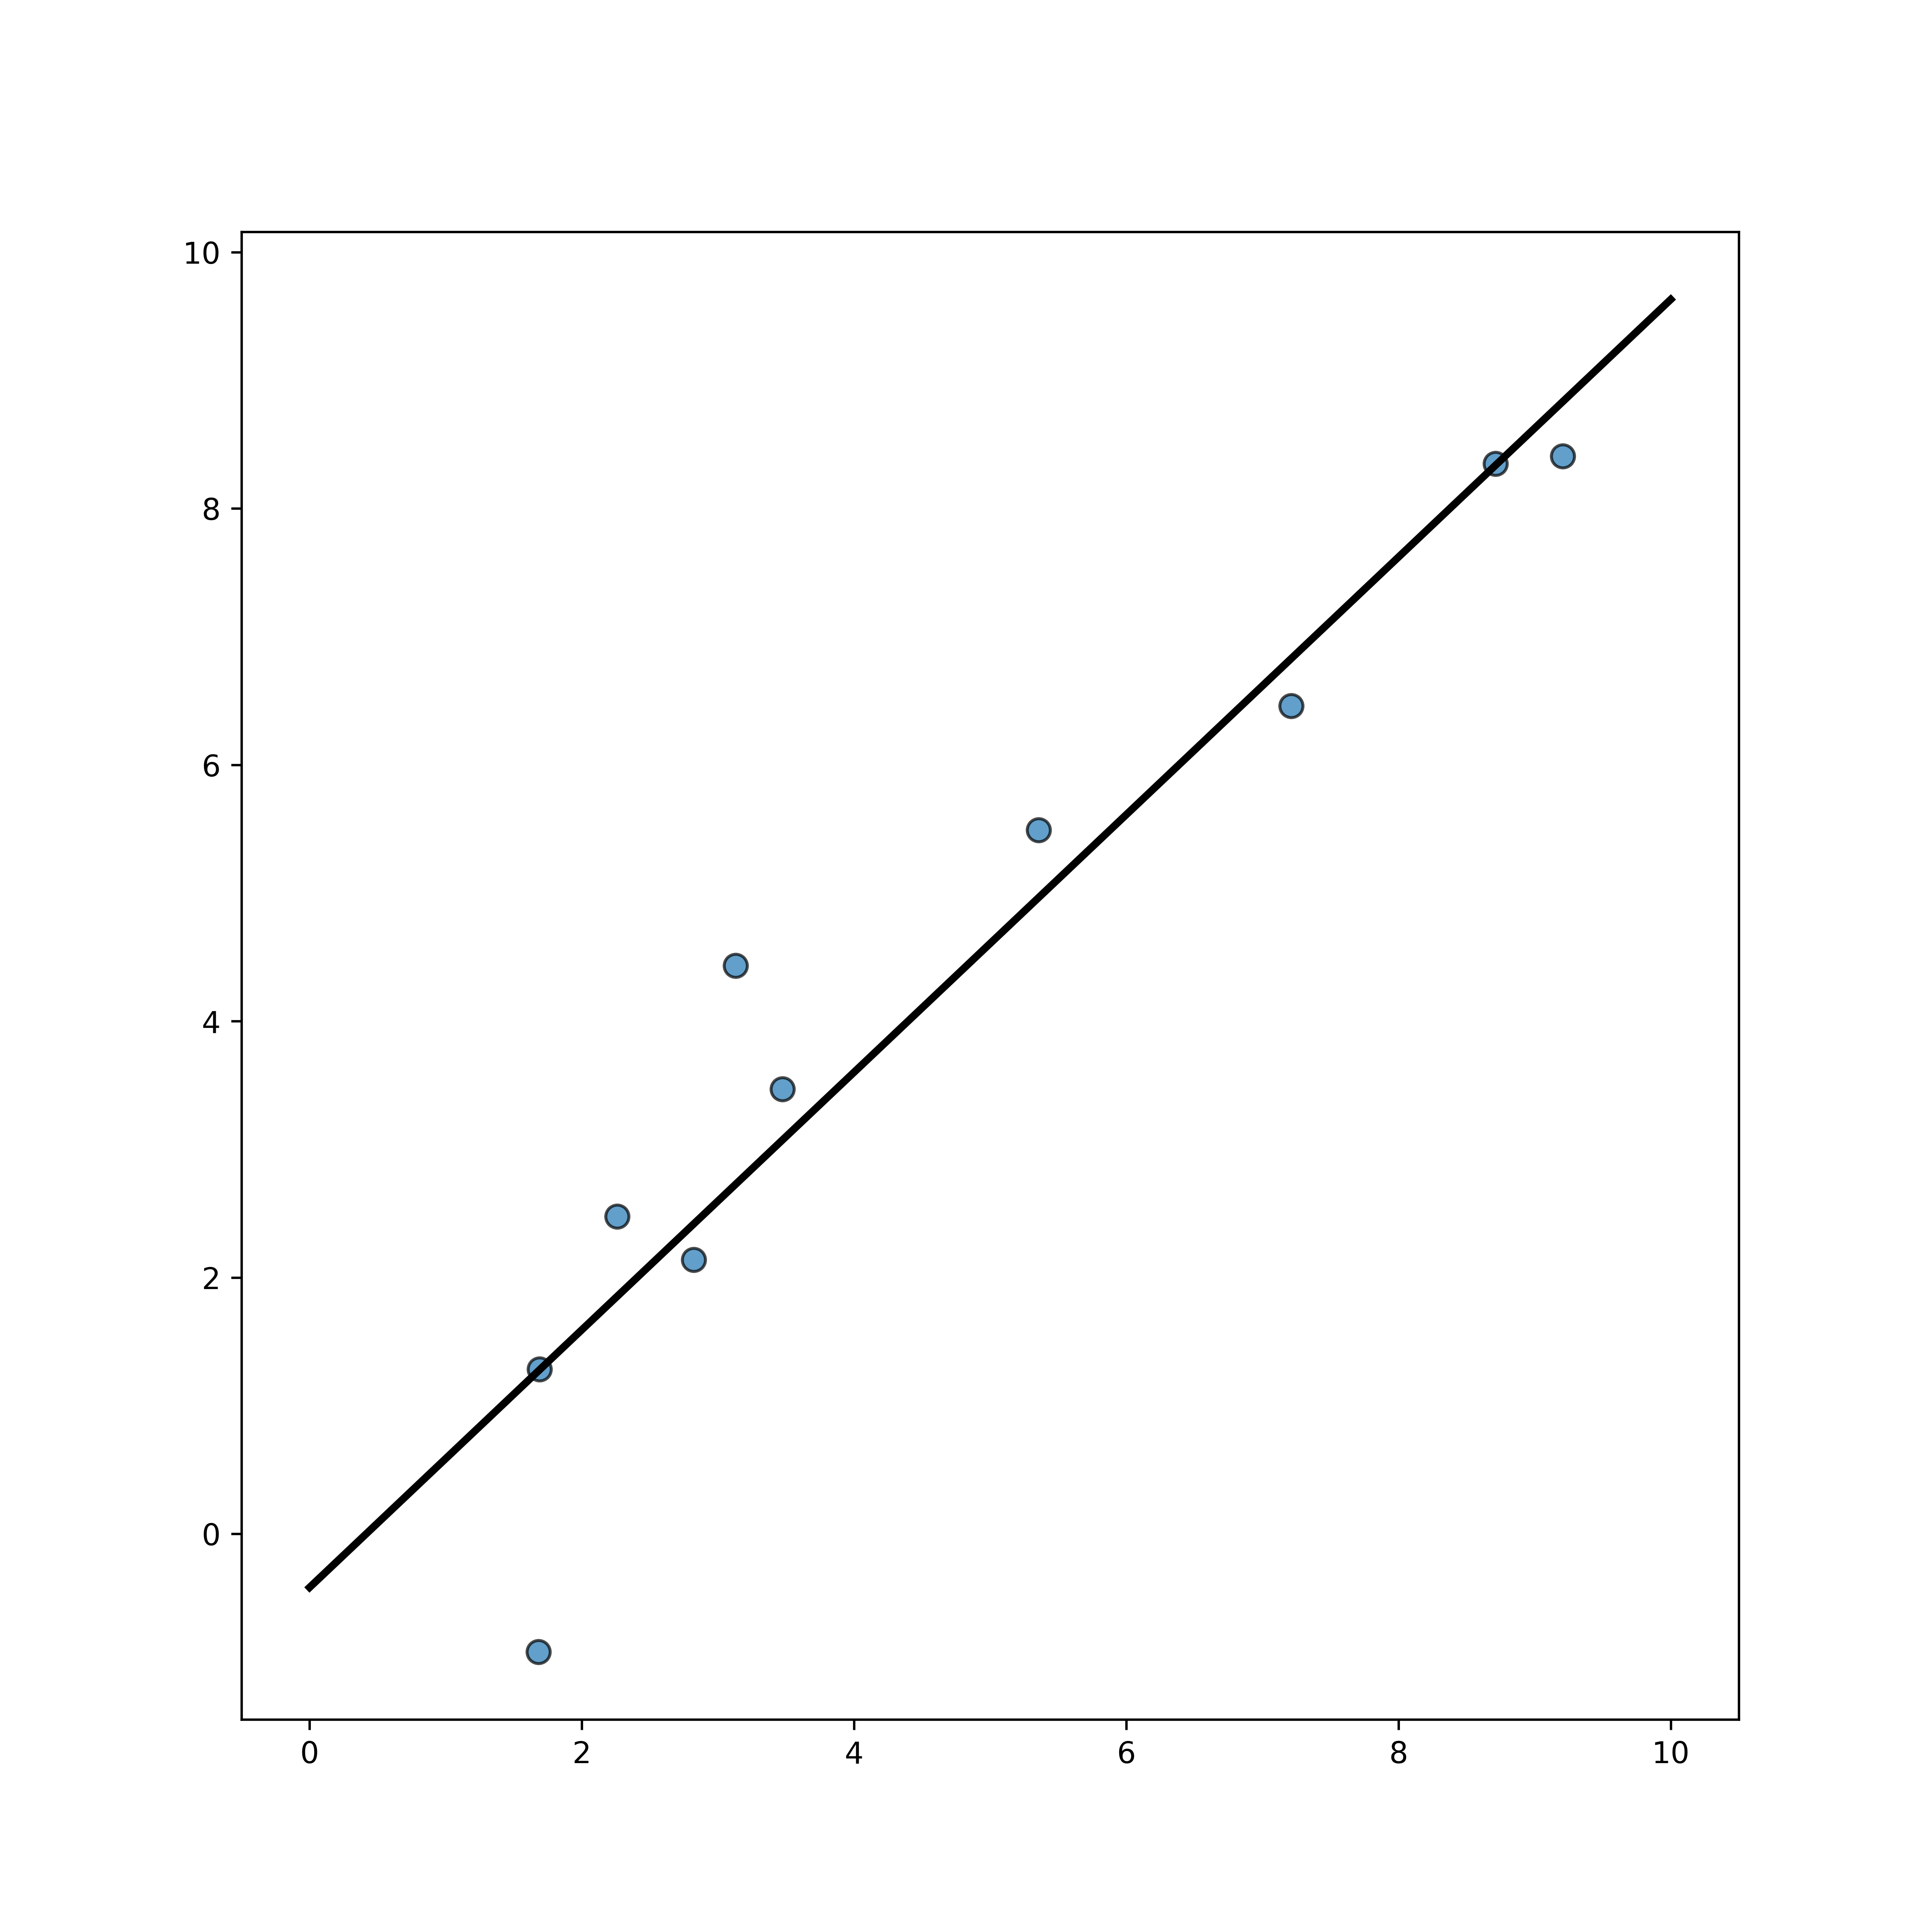
\includegraphics[width=0.6\textwidth]{images/lineplot.png}
    \end{center}
    }
\end{frame}

\begin{frame}{Problem Statement}
    Let $\forall i \in [n]: a_i \in \R^d, b_i\in \R$. Then find:
    $$
    \min_{x \in \R^d} \onslide<2->\underbrace{ \onslide<1->\frac{1}{n} \sum_{i=0}^n \onslide<3->\overbrace{ \onslide<1->  (a_i^T \cdot x -b_i)^2 \onslide<3->}^{\eqqcolon f_i(x)} \onslide<2-> }_{\eqqcolon g(x)}
    $$
\end{frame}

\section{FG}
\begin{frame}{(Full) Gradient Descent}
    How to solve such problem?
    \pause
    \begin{exampleblock}{Idea}
        Guess $x$, try to improve: go "down"\\
        \pause
        Formally: Guess $x^k$, set $x^{k+1} = x^k - \nabla g(x)$        
    \end{exampleblock}
    Called "Gradient Descent" or "Full Gradient"
\end{frame}

\subsection{local to global/convexity}
\begin{frame}{Properties of Full Gradient}
    \begin{block}{Notations}
        In the following let $x^*$ the optimal value,\pause
        $$ a \coloneqq \begin{pmatrix}- a_1^T - \\ \vdots \\ - a_n^T -\end{pmatrix}, \pause b \coloneqq \begin{pmatrix}b_1 \\ \vdots \\ b_n\end{pmatrix}$$
    \end{block} \vspace{-1.5pc} \pause
    \begin{alignat*}{3}
        \action<4->{ g(x) &= \sum_{i=1}^n \left( a_i^Tx - b_i \right)^2 &&= \|ax - b \|_2^2 \\
        } \action<5->{ \nabla g(x) &= \sum_{i=1}^n a_i \left( a_i^Tx - b_i \right) &&= a^T(ax-b) \\
        } \action<6>{ \pause \nabla^2 g(x) &= \sum_{i=1}^n a_i a_i^T &&= a^T a }
    \end{alignat*}
\end{frame}

\begin{frame}{$L$-smoothness}
    \begin{definition}[$L$-smoothness]
        Let $f: \R^d \to \R$ a function, $x_1, x_2 \in \R^d$.Then $f$ is called $L$-smooth if \pause $$\exists L : \| \nabla f(x_1) - \nabla f(x_2) \| \leq L \| x_1 - x_2 \|$$ \vspace{-1pc}
    \end{definition} 
    \pause
    \begin{proposition}
        The function $g$ from our problem is $L$-smooth.
    \end{proposition}
\end{frame}

\begin{frame}
    \begin{proof}
        Let $ x_1, x_2 \in \R^d, \, \pause B\coloneqq \max_{i \in [n]} \| a_i \|_2$. Then
        \begin{align*}
            \action<+->{\| \nabla g(x_1) - \nabla g(x_2) \| &= } \action<+->{ \| \sum_{i=1}^n a_i a_i^T (x_1 - x_2) \|_2\\ 
            &= } \action<+->{ \| a^T a (x_1 - x_2) \|_2 \\
            &\leq } \action<+->{ B^2 n \|(x_1 - x_2 )\| }
        \end{align*}
        \action<+->{ $\implies$ $g$ is $L$-smooth with $L \coloneqq B^2n$  }
    \end{proof}
    \action<+->{
    \begin{corollary}
        For $L$ from before it holds that 
        $$L = n \left( \max_{i \in [n]} \| a_i \|_2 \right)^2 \pause \geq \sigma_{max}(a^Ta)$$
    \end{corollary} }
\end{frame}

\begin{frame}{Properties}
    \begin{definition}[Convexity]
        Let $f: \R^d \to \R$ a function, $x_1, x_2 \in \R^d$.Then \pause
        \begin{enumerate}[label=(\roman*)]
            \item $f$ is called convex if $\forall 0 \leq t \leq 1$
            \begin{align*}
                \action<+->{ f(tx_1 + (1-t)x_2) &\leq \pause tf(x_1) + (1-t)f(x_2) \\ }\action<3->{
                \iff  f(x_1) &\geq f(x_2) + (\nabla f(x_2))^T (x_1 - x_2)}
            \end{align*} \vspace{-1pc} \action<4->{
            \item $f$ is called \textbf{strongly} convex if $$\exists \mu > 0 :  f(x_1) \geq \pause f(x_2) + (\nabla f(x_2))^T(x_1 - x_2) + \frac{\mu}{2} \| x_1 - x_2 \|_2^2$$ } \vspace{-1pc}
        \end{enumerate}
    \end{definition}
    \action<5->{Example: Blackboard}
\end{frame}

\begin{frame}{Local to Global}
    Why these Properties? \\ \pause
    \begin{enumerate}[label=-]
        \item Convex $\implies$ solution exists and is unique \pause
        \item Strongly convex $\implies$ small $g(x')$ is close to $g(x^*)$ implies $x'$ close to $x^*$ 
    \end{enumerate}    
\end{frame}

\begin{frame}
    \begin{theorem}
        The function $g$ from our problem is convex. \\ \pause
        If $\sigma_{min}(a^Ta) > 0$ it is even strongly convex
    \end{theorem}
\end{frame}

\begin{frame}
    \begin{proof} \vspace{-1pc}
        \begin{alignat*}{3}
            \action<+->{ &\overset{\text{Taylor}}{\implies} g(x') &&= g(x) + (\nabla g(x) )^T(x'-x) + \frac{1}{2}(x'-x)^Ta^Ta(x'-x)\\ } \action<2->{
            & &&\geq g(x) + (\nabla g(x) )^T(x'-x) + \frac{1}{2} \sigma_{min}(a^Ta) \|x'-x \|_2^2 } 
        \end{alignat*} \vspace{-1pc} \pause
        $$\implies g(x) + (\nabla g(x) )^T(x'-x) \leq g(x') - \frac{1}{2} \sigma_{min}(a^Ta) \|x'-x \|_2^2 $$\\ \pause
        $\implies$ g is strongly convex, if $\mu \coloneqq \sigma_{min}(a^Ta) > 0$
    \end{proof}
\end{frame}

\begin{frame}{Convergence rate}
    \begin{theorem}
        The FG method has for decreasing step size convergence rate of 
        $$g(x^k) - g(x^*) = \mathcal{O}(1/k)$$
        and \pause
        $$g(x^k) - g(x^*) = \mathcal{O}(\rho^k)$$
        if $g$ is strongly convex (i.e. $\sigma_{min}(a^Ta) > 0$
    \end{theorem}
\end{frame}

\subsection{Convergence}
\begin{frame}{Proof of convergence of FG}
    For the following, let $\eta_k$ the step size of every step, and 
    $$x_{k+1} \coloneqq x_k - \eta_k \nabla g(x_k)$$
    the update.\\ \pause
    Here: only strongly convex case
\end{frame}

\begin{frame}
    \begin{align*}
        \action<+->{ \| x_{k+1} - x^* \|_2^2 = &\langle x_{k+1} - x^*, x_{k+1} - x^* \rangle \\ 
            }\action<+->{ = &\langle x_k - \eta_k \nabla g(x_k) - x^*, x_k - \eta_k \nabla g(x_k) - x^* \rangle \\
            }\action<+->{ = &\langle x_k - x^*, x_k - \eta_k \nabla g(x_k) - x^* \rangle \\
            &- \langle \eta_k \nabla g(x_k), x_k - \eta_k \nabla g(x_k) - x^* \rangle \\
            }\action<+->{ = &\langle x_k - x^*, x_k  - x^* \rangle \\
            &- \langle \eta_k \nabla g(x_k), x_k - x^* \rangle \\
            &- \langle x_k - x^*, \eta_k \nabla g(x_k) \rangle \\
            &+ \langle \eta_k \nabla g(x_k), \eta_k \nabla g(x_k) \rangle \\
            }\action<+->{ = &\| x_{k} - x^* \|_2^2 - 2\eta_k(\nabla g(x_k))^T(x_k - x^*) + \eta_k^2 \| \nabla g(x_k) \|^2_2 }
    \end{align*}
\end{frame}

\begin{frame}
    \vspace{-0.5pc} Let $\delta_k \coloneqq g(x^*)-g(x_k)$ \vspace{-0.5pc}
    \begin{align*}
        \action<+->{ \| x_{k+1} - x^* \|_2^2 = } \action<+->{ &\| x_{k} - x^* \|_2^2 - 2\eta_k(\nabla g(x_k))^T(x_k - x^*)) + \eta_k^2 \| \nabla g(x_k) \|^2_2\\
        } \action<+->{ \leq &\| x_{k} - x^* \|_2^2 - 2\eta_k( g(x^*) - g(x_k) -\frac{\mu}{2} \| x_k - x^* \| ) \\
        &+ \eta_k^2 \| \nabla g(x_k) \|^2_2\\ \vspace{-1em}
        } \action<+->{ = &\|x_k-x^*\|_2^2(1-\eta_k\mu) - 2\eta_k\delta_k +\eta_k^2 \| \nabla g(x_k) \|^2_2 \\
        } \action<+->{ = & \|x_k-x^*\|_2^2(1-\eta_k\mu) - 2\eta_k\delta_k + \eta_k^2 \| \nabla g(x_k) - \nabla g(x^*) \|^2_2 \\ 
        } \action<+->{ \leq &\|x_k-x^*\|_2^2(1-\eta_k\mu) - 2\eta_k\delta_k + \eta_k^2 L^2\| x_k - x^* \|^2_2}
    \end{align*}
    \action<+->{Let $\eta_k \in (0, \min(\frac{\mu}{2L^2}, \frac{2}{\mu}) )$\\
    } \action<+->{$\implies \exists \rho \in (0,1) : \| x_k - x^* \|_2^2 \leq \rho^k \|x_0 - x^* \|^2_2$
    } \action<+->{$\implies g(x^*) - g(x_k) \leq \frac{1}{2} \rho^k \|x_0-x^*\|_2^2(\mu + \eta_k L^2) - \rho^{k+1} \frac{\| x_0 - x^* \|^2_2 }{2\eta_k}$\\
    } \action<+->{$\xrightarrow[]{}$Lyapunov function that controls convergence }
\end{frame}

\section{SG}
\begin{frame}{Where is the problem?}
    \begin{exampleblock}{Idea (FG)}
        Guess $x$, try to improve: go "down"\\
        Formally: Guess $x^k$, set $x^{k+1} = x^k - \eta_k \nabla g(x)$        
    \end{exampleblock}
    \pause
    But: $\nabla g(x) \in \R^d$\\
    \pause
    And: $[ \nabla g(x) ]_k = \frac{1}{n} \sum_{i=0}^n \nabla f_i(x)$ 
\end{frame}


\begin{frame}{A new challenger}
    \begin{alertblock}{Problem}
        $[ \nabla g(x) ]_k = \frac{1}{n} \sum_{i=0}^n \nabla f_i(x)$\\
        Calculating gradient of \textbf{all} samples
    \end{alertblock}
    \pause
    \begin{block}{Ansatz}
        Don't calculate the gradient for every sample. Go into "direction" of \textbf{one} sample
    \end{block}
    \pause
    \begin{exampleblock}{Formally}
        $x^{k+1} = x^k - \eta_k \nabla f_i(x)$
    \end{exampleblock}
    \pause
    But which $i$?
\end{frame}

\begin{frame}{Which $i$}
    \begin{block}{1. Idea}
        Just count 
        \pause 
        $\xrightarrow[]{}$ Samples could be ordered
    \end{block}
    \pause
    \begin{block}{2. Idea}
        Choose random one\\
        \pause
        Called "Stochastic gradient"
    \end{block}
\end{frame}

\subsection{convergence}
\begin{frame}{Convergence}
    \begin{block}{Theorem}
        For $k$ iterations, decreasing step size:
        $$\mathbb{E}[g(x^k)]-g(x^*) = \mathcal{O}(1/\sqrt{k})$$
        and
        \pause
        $$\mathbb{E}[g(x^k)]-g(x^*) = \mathcal{O}(1/k)$$
        if $g$ strongly-convex
    \end{block}
    \pause
    Can be shown similar as for FG.
\end{frame}

% \begin{frame}{Comparison to FG}
%     \begin{center}
%     \begin{tabular}{ c | c c }
%      & convex & strongly convex \\ 
%      \hline
%      FG & \only<2->{$\mathcal{O}(1/k)$} & \only<2->{$\mathcal{O}(\rho^k)$} \\  
%      SG & \only<3->{$\mathcal{O}(1/\sqrt{k})$} & \only<3->{$\mathcal{O}(1/k)$}    
%     \end{tabular}
%     \end{center}
%     \only<3->{For SG the convergence is in $\mathbb{E}$}
% \end{frame}

\section{SAG}
\begin{frame}{What about the other data?}
    SG Method does only consider \textbf{one} sample.\\
    \textbf{Question:} how to consider more without depending on the dimension?
    \pause
    \begin{exampleblock}{Idea}
        Take an average\\
        \pause
        Formally:
        $$x^{k+1} \coloneqq x^k - \frac{\alpha_k}{n}\sum_{i=0}^n y_i^k$$
        with
        \pause
        $$y_i^k \coloneqq \begin{cases}
            f'_i(x^k) & i = i_k\\
            y_i^{k-1} & else
        \end{cases}$$
        where $i_k$ is the random variable from the SG method.
    \end{exampleblock}
\end{frame}

\subsection{Theory}
\begin{frame}{Convergence}
    \begin{block}{Theorem 1}
        Let $L$ the Lipschitz constant of $g$, step size $\alpha_k \coloneqq\frac{1}{16L}$. The SAG method has convergence rate of:
        \pause
        $$\mathbb{E}[g(x^k)] - g(x^*) \leq \frac{32n}{k}C_0$$
        with \pause
        $$C_0 = \frac{3}{2} \left( g(x^0) - g(x^*) \right) + \frac{4L}{n}\| x^0 - x^* \|^2$$
        for $y_i^0=f'_i(x^0)-g'(x^0)$ and \pause
        $$\mathbb{E}[g(x^k)] - g(x^*) \leq \left( 1-min\left\{ \frac{\mu}{16L}, \frac{1}{8n} \right\} \right)^kC_0$$
        if $g$ strongly convex w.r.t. $\mu$.
    \end{block}
\end{frame}

\begin{frame}{Sketch of a proof}
    \textbf{Goal:} Want to find Lyapunov function again, s.th. it controls the convergence. \\ \pause
    $$\mathcal{L}: \R^d \to \R$$
    s.th. $\mathcal{L}(x) \geq \|x - x^*\|_2^2$. \pause
    For this, let
    $$y^k \coloneqq \begin{pmatrix} y_1^k \\ \vdots \\ y_n^k \end{pmatrix}, \theta^k \coloneqq \begin{pmatrix} y_1^k \\ \vdots \\ y_n^k \\ x^k \end{pmatrix}, \theta^* \coloneqq \begin{pmatrix}  f'_1(x^*) \\ \vdots \\ f'_n(x^*) \\ x^* \end{pmatrix}$$ and 
    $$e \coloneqq \begin{pmatrix} I \\ \vdots \\ I \end{pmatrix}, f'(x) \coloneqq \begin{pmatrix} f'_1(x) \\ \vdots \\ f'_n(x) \end{pmatrix}$$
\end{frame}
\begin{frame}
    \begin{block}{}
        Here the Lyapunov function has the following form:
        $$\mathcal{L}(\theta^k) = 2hg(x^k+de^Ty^k) - 2hg(x^*) + (\theta^k - \theta^*)^T\begin{pmatrix}
            A &B \\ B^T & C
        \end{pmatrix}(\theta^k - \theta^*)$$
    \end{block}
    \pause
    In the paper: solved by identifying coefficients, finding a valid ones with CAS.
\end{frame}

\begin{frame}
    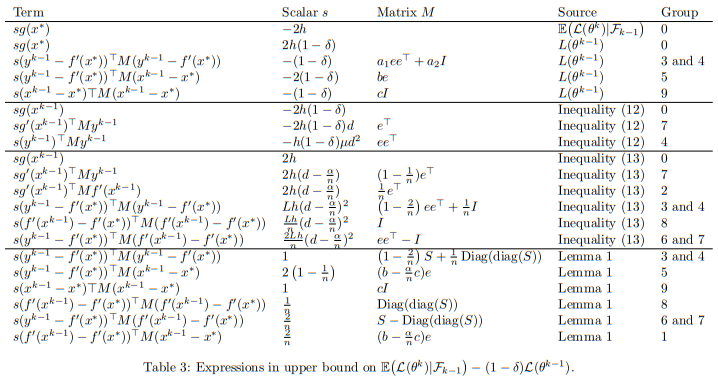
\includegraphics[width=\textwidth]{images/coefficients.png}
\end{frame}

\begin{frame}
    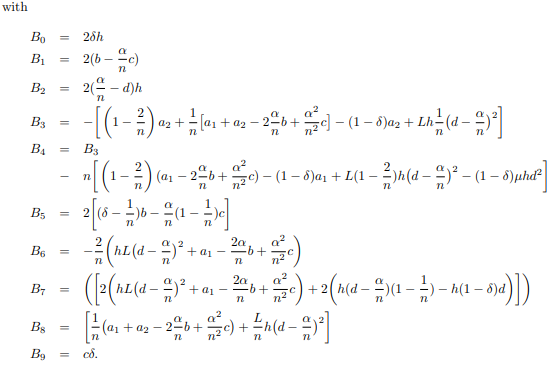
\includegraphics[width=\textwidth]{images/terms.png}
\end{frame}

\begin{frame}{A lemma}
    \begin{lemma}[2]
        Let $I\in \R^{p\times p}$ identity matrix, $e = \begin{pmatrix}I \\ \vdots \\ I\end{pmatrix}\in \R^{np \times p}$, $\alpha, \beta \in \R \setminus \{0\}$\\
        Then\pause
        $$ \left( \alpha \left( I - \frac{1}{n} ee^T \right) + \beta \left( \frac{1}{n} ee^T\right) \right)^{-1} = \frac{1}{\alpha} \left( I-\frac{1}{n} ee^T \right) + \frac{1}{\beta} \left( \frac{1}{n} ee^T \right) $$
    \end{lemma}\pause
    \begin{proof}
        First, notice that $e^Te = nI$. \pause Therefore we get $\left( \frac{1}{n} ee^T \right) \left( \frac{1}{n} ee^T \right) = \pause \frac{1}{n^2}e\underbrace{e^Te}_{=nI}e^T = \frac{1}{n} ee^T$ 
    \end{proof}
\end{frame}

\begin{frame}{A Lemma}
    \begin{align*}
    & \action<+->{\left( \alpha \left( I - \frac{1}{n} ee^T \right) + \beta \left( \frac{1}{n} ee^T\right) \right) \cdot \left( \frac{1}{\alpha} \left( I-\frac{1}{n} ee^T \right) + \frac{1}{\beta} \left( \frac{1}{n} ee^T \right) \right) \\ }\action<+->{
    = &\left( I - \frac{1}{n} ee^T \right)\left( I - \frac{1}{n} ee^T \right) 
    + }\action<+->{ \frac{\alpha}{\beta} \left( I - \frac{1}{n} ee^T \right)\left(\frac{1}{n} ee^T \right)\\
    &+ }\action<+->{ \frac{\beta}{\alpha} \left( \frac{1}{n} ee^T \right)\left(I-\frac{1}{n} ee^T \right)
    + }\action<+->{ \left( \frac{1}{n} ee^T \right)\left( \frac{1}{n} ee^T \right)\\
    = }\action<+->{ &\left( I - \frac{2}{n} ee^T + \frac{1}{n}ee^T \right) 
    + }\action<+->{ \frac{\alpha}{\beta} \left( \frac{1}{n} ee^T - \frac{1}{n} ee^T \right) \\
    &+ }\action<+->{ \frac{\beta}{\alpha} \left( \frac{1}{n} ee^T - \frac{1}{n} ee^T \right) 
    + }\action<+->{ \frac{1}{n} ee^T  \\
    =& I \qed}
    \end{align*}
\end{frame}

\begin{frame}{Comparison to FG}
    \begin{center}
    \begin{tabular}{ c | c c }
     & convex & strongly convex \\ 
     \hline
     FG & $\mathcal{O}(1/k)$ & $\mathcal{O}(\rho^k)$ \\  
     SG & $\mathcal{O}(1/\sqrt{k})$ & $\mathcal{O}(1/k)$\\
     SAG & &
    \end{tabular}
    \end{center}
    \only<2->{For SG and SAG the convergence is in $\mathbb{E}$}
\end{frame}

\section{Alg.}
\begin{frame}{Basic Algorithm}
    The basic Algorithm just updates every time with $$x^{k+1} = x^k - \frac{\alpha_k}{n}\sum_{i=1}^ny_i^k$$
    \pause
    Potential improvements are:
    \begin{enumerate}[label=-]
        \item Just in time parameter updates \pause
        \item Adding weigths to already seen samples \pause
        \item Warm starting \pause
        \item Line-searching $L$ \pause
        \item Mini-batches
    \end{enumerate}
\end{frame}

\section{Experiments}
\begin{frame}{Experimental results}
    \begin{block}{Dataset}
        KDD Cup 2004\\
        50.000 samples, 78 features/dimensions
    \end{block}
    Logistic regression, with same learning rate for all algorithms
\end{frame}



\end{document}
